\documentclass[crop=false]{standalone}
%\documentclass{standalone}
\usepackage{tikz} % To generate the plot from csv
\usepackage{pgfplots}
\usepackage{graphicx}
\usepackage{booktabs}
\usepackage{subfig}
\usepackage{float}
\usepackage[section]{placeins} % getting figures below sections
\usepackage{blindtext}
\usepackage{siunitx}
\usepgfplotslibrary{units} % Allows to enter the units nicely
\usetikzlibrary{external} %https://tex.stackexchange.com/questions/1460/script-to-automate-externalizing-tikz-graphics
\tikzexternalize[prefix=savedfigures/]

\pgfplotsset{compat=newest} % Allows to place the legend below plot
\usepackage{pgfplotstable}
\usepgfplotslibrary{statistics}

% #################### Function definition for box plots read table ##################\
\makeatletter
\pgfplotsset{
	boxplot prepared from table/.code={
		\def\tikz@plot@handler{\pgfplotsplothandlerboxplotprepared}%
		\pgfplotsset{
			/pgfplots/boxplot prepared from table/.cd,
			#1,
		}
	},
	/pgfplots/boxplot prepared from table/.cd,
	table/.code={\pgfplotstablecopy{#1}\to\boxplot@datatable},
	row/.initial=0,
	make style readable from table/.style={
		#1/.code={
			\pgfplotstablegetelem{\pgfkeysvalueof{/pgfplots/boxplot prepared from table/row}}{##1}\of\boxplot@datatable
			\pgfplotsset{boxplot/#1/.expand once={\pgfplotsretval}}
		}
	},
	make style readable from table=lower whisker,
	make style readable from table=upper whisker,
	make style readable from table=lower quartile,
	make style readable from table=upper quartile,
	make style readable from table=median,
	make style readable from table=average,
	make style readable from table=lower notch,
	make style readable from table=upper notch
}
\makeatother
\begin{document}

\section{3 3 Mumford1 GA Mutations 20210718 131331}

% ######################## UTRP GA Mutation operators applied ######################## 
\begin{figure} 
\centering 
\tikzsetnextfilename{UTRP_NSGAII_BP_mutation_funcs} 
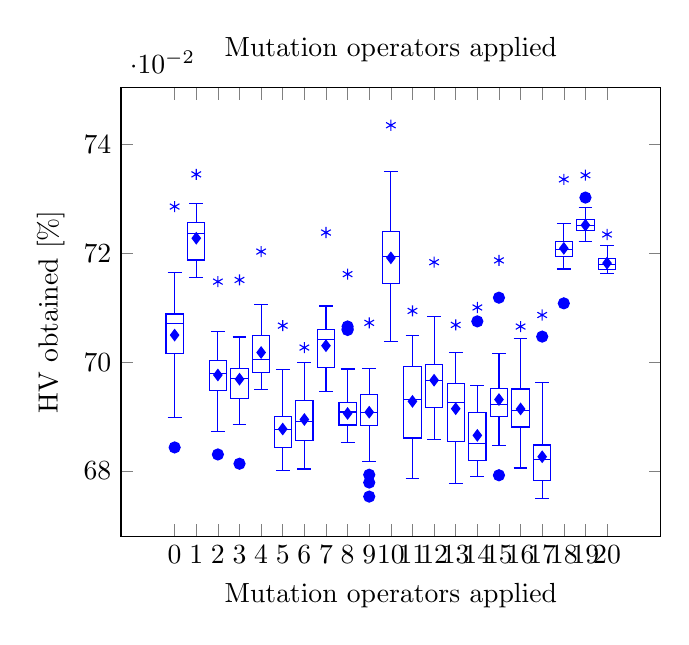
\begin{tikzpicture} 
\begin{axis}[ 
title={Mutation operators applied}, 
boxplot/draw direction=y, 
xtick={1,2,3,4,5,6,7,8,9,10,11,12,13,14,15,16,17,18,19,20,21}, 
xticklabels={0,1,2,3,4,5,6,7,8,9,10,11,12,13,14,15,16,17,18,19,20}, 
x tick label style={rotate=0, align=center}, 
xlabel={Mutation operators applied}, 
scaled y ticks={base 10:2}, %y tick label style={/pgf/number format/.cd,fixed,precision=3, zerofill}, 
ylabel={HV obtained [\%]}, 
] 

% ############## Mutations=0 ################## 
\addplot[boxplot, mark=*, 
boxplot prepared={ 
lower whisker=0.68991, 
upper whisker=0.71641, 
lower quartile=0.70159, 
upper quartile=0.70885, 
median=0.70712, 
average=0.70498}, 
color = blue, solid, area legend] 
coordinates {
(1,0.68434)}; 
\addplot[only marks,mark=asterisk,color = blue]coordinates{(1,0.72859)}; 

% ############## Mutations=1 ################## 
\addplot[boxplot, mark=*, 
boxplot prepared={ 
lower whisker=0.7156, 
upper whisker=0.72922, 
lower quartile=0.71877, 
upper quartile=0.72559, 
median=0.72358, 
average=0.72278}, 
color = blue, solid, area legend] 
coordinates {}; 
\addplot[only marks,mark=asterisk,color = blue]coordinates{(2,0.73451)}; 

% ############## Mutations=2 ################## 
\addplot[boxplot, mark=*, 
boxplot prepared={ 
lower whisker=0.68727, 
upper whisker=0.7056, 
lower quartile=0.69481, 
upper quartile=0.70033, 
median=0.69796, 
average=0.69765}, 
color = blue, solid, area legend] 
coordinates {
(3,0.68305)}; 
\addplot[only marks,mark=asterisk,color = blue]coordinates{(3,0.7148)}; 

% ############## Mutations=3 ################## 
\addplot[boxplot, mark=*, 
boxplot prepared={ 
lower whisker=0.68851, 
upper whisker=0.70462, 
lower quartile=0.69336, 
upper quartile=0.69879, 
median=0.69701, 
average=0.69688}, 
color = blue, solid, area legend] 
coordinates {
(4,0.68135)}; 
\addplot[only marks,mark=asterisk,color = blue]coordinates{(4,0.71511)}; 

% ############## Mutations=4 ################## 
\addplot[boxplot, mark=*, 
boxplot prepared={ 
lower whisker=0.69501, 
upper whisker=0.71056, 
lower quartile=0.69818, 
upper quartile=0.7049, 
median=0.70056, 
average=0.70178}, 
color = blue, solid, area legend] 
coordinates {}; 
\addplot[only marks,mark=asterisk,color = blue]coordinates{(5,0.72032)}; 

% ############## Mutations=5 ################## 
\addplot[boxplot, mark=*, 
boxplot prepared={ 
lower whisker=0.68014, 
upper whisker=0.69858, 
lower quartile=0.68433, 
upper quartile=0.69003, 
median=0.68756, 
average=0.68772}, 
color = blue, solid, area legend] 
coordinates {}; 
\addplot[only marks,mark=asterisk,color = blue]coordinates{(6,0.70672)}; 

% ############## Mutations=6 ################## 
\addplot[boxplot, mark=*, 
boxplot prepared={ 
lower whisker=0.68037, 
upper whisker=0.69997, 
lower quartile=0.68555, 
upper quartile=0.69302, 
median=0.68916, 
average=0.68947}, 
color = blue, solid, area legend] 
coordinates {}; 
\addplot[only marks,mark=asterisk,color = blue]coordinates{(7,0.70269)}; 

% ############## Mutations=7 ################## 
\addplot[boxplot, mark=*, 
boxplot prepared={ 
lower whisker=0.69457, 
upper whisker=0.71032, 
lower quartile=0.69896, 
upper quartile=0.70604, 
median=0.70419, 
average=0.70303}, 
color = blue, solid, area legend] 
coordinates {}; 
\addplot[only marks,mark=asterisk,color = blue]coordinates{(8,0.72382)}; 

% ############## Mutations=8 ################## 
\addplot[boxplot, mark=*, 
boxplot prepared={ 
lower whisker=0.68517, 
upper whisker=0.69874, 
lower quartile=0.68846, 
upper quartile=0.69263, 
median=0.69085, 
average=0.69058}, 
color = blue, solid, area legend] 
coordinates {
(9,0.70592)
(9,0.70609)
(9,0.70656)}; 
\addplot[only marks,mark=asterisk,color = blue]coordinates{(9,0.71618)}; 

% ############## Mutations=9 ################## 
\addplot[boxplot, mark=*, 
boxplot prepared={ 
lower whisker=0.68175, 
upper whisker=0.69884, 
lower quartile=0.68839, 
upper quartile=0.69412, 
median=0.69075, 
average=0.69081}, 
color = blue, solid, area legend] 
coordinates {
(10,0.67789)
(10,0.67932)
(10,0.67531)}; 
\addplot[only marks,mark=asterisk,color = blue]coordinates{(10,0.70723)}; 

% ############## Mutations=10 ################## 
\addplot[boxplot, mark=*, 
boxplot prepared={ 
lower whisker=0.70386, 
upper whisker=0.7351, 
lower quartile=0.71446, 
upper quartile=0.72403, 
median=0.71944, 
average=0.71917}, 
color = blue, solid, area legend] 
coordinates {}; 
\addplot[only marks,mark=asterisk,color = blue]coordinates{(11,0.74353)}; 

% ############## Mutations=11 ################## 
\addplot[boxplot, mark=*, 
boxplot prepared={ 
lower whisker=0.67869, 
upper whisker=0.7049, 
lower quartile=0.68607, 
upper quartile=0.69924, 
median=0.69309, 
average=0.6928}, 
color = blue, solid, area legend] 
coordinates {}; 
\addplot[only marks,mark=asterisk,color = blue]coordinates{(12,0.70942)}; 

% ############## Mutations=12 ################## 
\addplot[boxplot, mark=*, 
boxplot prepared={ 
lower whisker=0.68581, 
upper whisker=0.70841, 
lower quartile=0.69161, 
upper quartile=0.69957, 
median=0.69667, 
average=0.69669}, 
color = blue, solid, area legend] 
coordinates {}; 
\addplot[only marks,mark=asterisk,color = blue]coordinates{(13,0.71837)}; 

% ############## Mutations=13 ################## 
\addplot[boxplot, mark=*, 
boxplot prepared={ 
lower whisker=0.67764, 
upper whisker=0.70186, 
lower quartile=0.6854, 
upper quartile=0.69602, 
median=0.69254, 
average=0.69145}, 
color = blue, solid, area legend] 
coordinates {}; 
\addplot[only marks,mark=asterisk,color = blue]coordinates{(14,0.70685)}; 

% ############## Mutations=14 ################## 
\addplot[boxplot, mark=*, 
boxplot prepared={ 
lower whisker=0.67898, 
upper whisker=0.6957, 
lower quartile=0.68197, 
upper quartile=0.69072, 
median=0.68512, 
average=0.68656}, 
color = blue, solid, area legend] 
coordinates {
(15,0.7075)}; 
\addplot[only marks,mark=asterisk,color = blue]coordinates{(15,0.71005)}; 

% ############## Mutations=15 ################## 
\addplot[boxplot, mark=*, 
boxplot prepared={ 
lower whisker=0.68463, 
upper whisker=0.7016, 
lower quartile=0.69, 
upper quartile=0.69509, 
median=0.69216, 
average=0.69314}, 
color = blue, solid, area legend] 
coordinates {
(16,0.71185)
(16,0.67923)}; 
\addplot[only marks,mark=asterisk,color = blue]coordinates{(16,0.7187)}; 

% ############## Mutations=16 ################## 
\addplot[boxplot, mark=*, 
boxplot prepared={ 
lower whisker=0.68056, 
upper whisker=0.70432, 
lower quartile=0.68809, 
upper quartile=0.69507, 
median=0.69108, 
average=0.69141}, 
color = blue, solid, area legend] 
coordinates {}; 
\addplot[only marks,mark=asterisk,color = blue]coordinates{(17,0.70655)}; 

% ############## Mutations=17 ################## 
\addplot[boxplot, mark=*, 
boxplot prepared={ 
lower whisker=0.6749, 
upper whisker=0.69625, 
lower quartile=0.67831, 
upper quartile=0.68479, 
median=0.68219, 
average=0.68263}, 
color = blue, solid, area legend] 
coordinates {
(18,0.7047)}; 
\addplot[only marks,mark=asterisk,color = blue]coordinates{(18,0.70867)}; 

% ############## Mutations=18 ################## 
\addplot[boxplot, mark=*, 
boxplot prepared={ 
lower whisker=0.71712, 
upper whisker=0.7254, 
lower quartile=0.71936, 
upper quartile=0.72222, 
median=0.72068, 
average=0.72092}, 
color = blue, solid, area legend] 
coordinates {
(19,0.71081)}; 
\addplot[only marks,mark=asterisk,color = blue]coordinates{(19,0.73359)}; 

% ############## Mutations=19 ################## 
\addplot[boxplot, mark=*, 
boxplot prepared={ 
lower whisker=0.7222, 
upper whisker=0.72845, 
lower quartile=0.72414, 
upper quartile=0.72615, 
median=0.72504, 
average=0.72517}, 
color = blue, solid, area legend] 
coordinates {
(20,0.73024)}; 
\addplot[only marks,mark=asterisk,color = blue]coordinates{(20,0.73435)}; 

% ############## Mutations=20 ################## 
\addplot[boxplot, mark=*, 
boxplot prepared={ 
lower whisker=0.71625, 
upper whisker=0.72137, 
lower quartile=0.71704, 
upper quartile=0.71911, 
median=0.718, 
average=0.7182}, 
color = blue, solid, area legend] 
coordinates {}; 
\addplot[only marks,mark=asterisk,color = blue]coordinates{(21,0.72346)}; 

\end{axis}
\end{tikzpicture}
\end{figure} 
\begin{table}
\centering
\caption{Legend for the boxplot.}
\begin{tabular}{ll}
\toprule
 Index &                      Name \\
\midrule
     0 &          [Intertwine\_two] \\
     1 &              [Add\_vertex] \\
     2 &           [Delete\_vertex] \\
     3 &    [Invert\_path\_vertices] \\
     4 &    [Insert\_inside\_vertex] \\
     5 &    [Delete\_inside\_vertex] \\
     6 &  [Relocate\_inside\_vertex] \\
     7 &   [Replace\_inside\_vertex] \\
     8 &   [Donate\_between\_routes] \\
     9 &     [Swap\_between\_routes] \\
    10 &         [Merge\_terminals] \\
    11 &      [Repl\_low\_dem\_route] \\
    12 &    [Rem\_low\_dem\_terminal] \\
    13 &   [Rem\_lrg\_cost\_terminal] \\
    14 &            [Repl\_subsets] \\
    15 &    [Trim\_one\_terminal\_cb] \\
    16 & [Trim\_one\_path\_random\_cb] \\
    17 &   [Trim\_routes\_random\_cb] \\
    18 &    [Grow\_one\_terminal\_cb] \\
    19 & [Grow\_one\_path\_random\_cb] \\
    20 &   [Grow\_routes\_random\_cb] \\
\bottomrule
\end{tabular}
\end{table}

\end{document}
